% !TEX root = memoire/main.tex

\chapter{Assimilation de données pour la construction d'un jumeau numérique}~\label{sec:da}

\section{Introduction}~\label{sec:intro_da}

La construction d'un système expert ou jumeau numérique a besoin de méthodes qui puissent faire le lien entre observations et l'état de notre simulation. En effet, les solutions calculées par les modèles numériques comportent des erreurs qu'il est crucial de comprendre, de quantifier et de réduire. Cette incertitude peut se manifester sous diverses formes, telles que l'ambiguïté des valeurs des paramètres du modèle, l'imprécision des conditions initiales, ou l'incertitude dans la définition des conditions aux limites ou des forces extérieures. De plus, bien que les modèles numériques intègrent généralement des principes physiques essentiels, ils impliquent certaines simplifications. L'erreur numérique apparaît en raison de l'algorithme et de la discrétisation. Elle s'étend également à l'incertitude associée aux futures mesures expérimentales calibrant les modèles numériques. Ainsi, les méthodes d'assimilation de données sont mises en place pour combiner les informations issues d'un modèle numérique, et celles issues de l'observation, et ce, de manière optimale, c'est-à-dire en tenant compte de leurs incertitudes respectives.

L'intégration des prévisions des modèles et des données d'observation a été largement appliquée dans des disciplines telles que la météorologie, l'océanographie, et les géosciences~\cite{bocquet_introduction_2014}. Dans le domaine de l'assimilation de données, deux grandes familles d'approche émerge :

\begin{itemize}
    \item les \textbf{méthodes séquentielles stochastiques} cherchent à estimer la distribution à chaque nouvelle acquisition d'une observation au travers du filtrage Bayésien. On trouve principalement le filtre de Kalman~\cite{kalman_new_1960} et ses variantes ainsi que les méthodes de Monte-Carlo séquentielles ;
    \item les \textbf{méthodes variationnelles} cherchent à estimer l'estimateur de maximum a posteriori par la minimisation d'une fonction de coût~\cite{variational_method}. Les formulations les plus courantes dérivent des méthodes 3D-Var et 4D-Var~\cite{talagrand1997assimilation}.
\end{itemize}


Dans ce chapitre, nous présenterons la formulation du problème d'assimilation sous sa forme probabiliste. Nous présenterons ensuite certaines méthodes stochastiques et variationnelles ainsi que leurs extensions d'ensemble que nous utiliserons dans les chapitres suivants. Pour des explications plus détaillées, veuillez vous référer à la bibliographie~\cite{law_data_2015,asch_data_2016,evensen_data_2022}.

% Les approches stochastiques séquentielles cherchent à estimer la distribution à chaques nouvelles acquisitions d'une observation. Dans ce cas, c'est la distribution de l'état elle-même qui est approchée. Le processus d'assimilation est réalisé dans un cadre Bayésien avec une étape de prévision et une étape d'analyse. Le filtre de Kalman~\cite{kalman_new_1960} est un exemple de formulation séquentielle considérant un modèle linéaire et des hypothèses de distribution Gaussienne. Des filtres plus avancés ont été introduits pour s'adapter aux distributions non linéaires et arbitraires. L'un des filtres les plus populaires est sans aucun doute le filtre de Kalman d'ensemble, introduit par Evensen~\cite{evensen_sequential_1994}, principalement en raison de son adaptabilité aux problèmes de grande dimension avec n'importe quel modèle d'évolution et de sa résilience aux écarts par rapport aux hypothèses Gaussiennes initiales. Il consiste à approximer la distribution de probabilité d'un état grâce à un ensemble de simulations appelées particules ou membres.
% Les approches variationnelles~\cite{variational_method} se concentrent sur la minimisation d'une fonction de coût qui mesure le décalage entre les prévisions du modèle et les observations, cherchant ainsi l'état optimal du système. Les formulations les plus courantes dérivent des méthodes 3D-Var et 4D-Var~\cite{talagrand1997assimilation}.

% Dans ce chapitre nous présenterons le formalisme pour l'assimilation de données ainsi que certaines méthodes stochastiques et variationnelles ainsi que leurs extensions ensemblistes.
\section{Formulation du problème}

\begin{definition}[assimilation de données]
    Par \textit{assimilation de données}, nous entendons toutes les méthodes et algorithmes qui permettent d’estimer l’\textbf{état} d’un système, à l’aide d’un \textbf{modèle} mathématique décrivant son évolution, des \textbf{observations} disponibles, des statistiques décrivant les \textbf{erreurs}, et de toute autre information possible sur cet état.
\end{definition}

Nous présentons l'ensemble des termes de cette définition.

\subsection{Définition de l'état}

Nous définissons un état $\bm z_k$ comme la variable qui représente complètement la connaissance du système à l'instant $t_k \in \mathbb R^+$. La dynamique de l'état du système au cours du temps est obtenue grâce à un modèle $\mathcal{M}$ qui décrit l'évolution du système.
Nous noterons $\mathcal Z_k = \{\bz_0, \dots, \bz_k\}$ la trajectoire du modèle jusqu'au pas de temps $t_k$.
Nous supposerons que le modèle admet des incertitudes. Celle-ci sont issues de

\begin{itemize}
    \item \textbf{L'erreur de discrétisation} dans l'espace et le temps. Soit $\bz^c$ l'état réel continu. Le modèle numérique ne traite que des représentations discrètes du champ physique. Ainsi, c'est non pas l'état $\bm x^c$ qui est estimé mais une projection dans l'espace de discrétisation. On estimera $\bz^t = \Pi(\bz^c)$, où $\Pi$ est un projecteur sur l'espace de discrétisation. On parle ici d'erreur de représentativité.
    \item \textbf{L'erreur de modèle}. C'est un modèle numérique qui calcule l'évolution de l'état simulé. Tout modèle étant imparfait, toutes les physiques ne peuvent êter prises en compte. C'est une erreur qui tient compte de la mauvaise représentation de l'évolution du système, mais également de sa discrétisation.
    \item \textbf{L'erreur de données} Le modèle mathématique doit être complété par des données et des paramètres spécifiant les caractéristiques physiques du système simulé parmi la classe des systèmes représentés par le modèle. Ces données peuvent concerner la géométrie du système, les conditions aux limites et initiales, ainsi que les forçages externes. Les paramètres peuvent être des constantes physiques ou des constantes du modèle prescrivant les lois constitutives du système. L'utilisation de données qui ne reflètent que partiellement la nature du système exact induit des erreurs supplémentaires, appelées erreurs de données, sur la prédiction.
\end{itemize}

Ainsi, nous traiterons l'état comme une variable aléatoire tel que à laquelle nous lui associerons une incertitude à la prédiction $\bm \eta_k$

\begin{equation*}
    \mathcal Z_k = \mathcal{M}(\bz_0, t_k ; \bm \theta) + \bm \eta_k.
\end{equation*}
où $\bm \theta$ sont l'ensemble des paramètres du modèle et $\bm z_0$ l'état initial.

\subsection{Définition des observations}
A l'équation d'évolution, nous supposons également connu une équation d'observation. Celle-ci relie l'état à l'espace de mesures. On définie $\mathcal{D}_k$ les mesures prédites par la fenêtre d'état $\mathcal{Z}_k$. Tout comme l'état, les mesures sont sujettes à des incertitudes issues de plusieurs sources

\begin{itemize}
    \item \textbf{L'erreur de mesure}. L'observable $\bm y^c$ est issue d'un signal réel fonction de l'état continu $\bm x^c$. Or ce signal est mesuré par une capteur sujet à des erreurs instrumentales $\bm \varepsilon^{\mu}$. C'est une erreur intrinsèque à la méthode d'acquisition et tient compte par exemple d'interférences environnementales, du bruit électronique, ou des biais systématiques des capteurs.
    \item \textbf{L'erreur de représentativité}. L'observation est prédite par un opérateur d'observation numérique $\mathcal H$ via $\bm x_k$. Ainsi, une erreur supplémentaire est induite par la représentation de l'opérateur $\mathcal H$ et celle de la projection de l'état continu avec $\Pi$. Par exemple, la discrétisation du modèle numérique ne peut pas représenter fidèlement les plus petites échelles spatiales ou temporelles présentes dans le système réel. Cette limitation entraîne une perte d'information et une simplification excessive des dynamiques fines, ce qui peut impacter directement les résultats de prédiction d'observation.
\end{itemize}

En supposant que ces erreurs sont additives, on défini la formule suivante
\begin{equation*}
    \mathcal D_k = \mathcal H (\mathcal{Z}_k) + \bm{\varepsilon}_k
\end{equation*} où $\bm{\varepsilon}_k = \bm{\varepsilon}^\mu  + \bm{\varepsilon}^r$ défini l'incertitude sur l'observation $\mathcal D_k$ relatif à la prédiction $\mathcal{Z}_k$.

\subsection{Inférence Bayésienne récursive}

Le problème d'assimilation de données peut être formulé sous une approche d'inférence Bayésienne. Celle-ci est une méthode statistique pour estimer l'état $\mathcal Z_k$ en utilisant à la fois une information a priori, obtenue à partir d'un modèles et des connaissances initiales, et les données observées. Cette méthode repose sur le théorème de Bayes qui décrit la relation entre la distribution a posteriori de l'état étant donné les données observées avec $p(\mathcal Z_k \mid \mathcal D_k)$ la distribution a priori de l'état $p(\mathcal Z_k)$ et la vraisemblance des données $p(\mathcal D_k \mid \mathcal Z_k)$ conditionnellement à l'état. Cette formule est la suivante
\begin{equation*}
    p(\mathcal Z_k \mid \mathcal D_k) = \frac{(\mathcal D_k \mid \mathcal Z_k)~p(\mathcal Z_k)}{p(\mathcal D_k)},
\end{equation*}où $p(\mathcal D_k)$  est la distribution marginale des observations. Elle agit comme constante de normalisation afin d'assurer que l'intégrale de la distribution a posteriori soit égale à 1.

% \begin{equation*}
%     p(\mathcal D_k) = \mathbb E_{\mathcal Z_k}[\mathcal D_k \mid \mathcal Z_k]
% \end{equation*}

Nous souhaitons résoudre le problème d'assimilation de manière séquentielle. C'est-à-dire, mettre à jour l'état à chaque nouvelle observation à l'instant $t_k$. Pour ce faire, nous utilisons deux approximations

\begin{itemize}
    \item Le modèle dynamique est une \textbf{chaîne de Markov d'odre 1}. Cette hypothèse suppose que l'état futur $\bm z_{k+1}$ est indépendant des états passés $\mathcal Z_{k-1}$ conditionnellement à l'état présent $\bm z_{k}$. Le modèle dynamique s'écrit alors

          \begin{equation*}
              \bm z_k = \mathcal{M}(\bz_{k-1} ; \bm \theta) + \bm \eta_k,
          \end{equation*}ce qui implique que
          \begin{equation*}
              p(\bz_{k+1} \mid \bz_{k},\bz_{k-1}\dots \bz_{0}) = p(\bz_{k+1} \mid \bz_{k}).
          \end{equation*}

          Ainsi, la probabilité de l'état $p(\mathcal{Z}_k)=p(\bz_0, \dots, \bz_k)$ devient

          \begin{eqnarray*}
              p(\mathcal{Z}_k) &=& p(\bz_0) p(\bz_1 \mid \bz_0) p(\bz_2 \mid \bz_1) \dots p(\bz_k \mid \bz_{k-1}) \\
              &=& p(\bz_0) \prod_{l = 1}^{k} p(\bz_l \mid \bz_{l-1}).
          \end{eqnarray*}

    \item Les observations sont indépendantes entre chaque assimilation. Cette hypothèse suppose que les observations présentes $\by_k$ soit indépendante des états et observations passé conditionnellement à $\bz_k$. Ceci correspond à définir une loi d'émission locale
          \begin{equation*}
              \by_k = \mathcal H (\bz_k) + \bm{\varepsilon}_k
          \end{equation*}
          ainsi qu'une vraisemblance comme le produit de vraisemblance locale
          \begin{equation*}
              p(\mathcal{D}_k \mid \mathcal Z_k) = \prod_{l=1}^{k} p(\by_l \mid \bx_l)
          \end{equation*}
\end{itemize}

Ainsi la trajectoire de l'état et des observation suis les hypothèses d'un modèle de Markov cachés, ici à temps discret, et qui peut être schématisé par le schéma Figure~\ref{fig:hidden_markov}.

\begin{figure}[h]
    \centering
    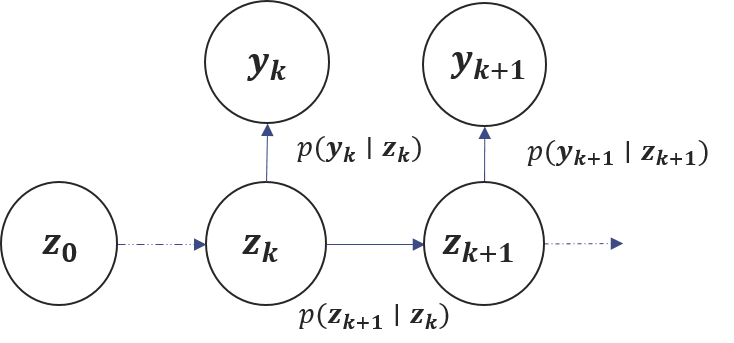
\includegraphics[width=0.5\textwidth]{hmc.png}
    \caption{Chaîne de Markov cachée}
    \label{fig:hidden_markov}
\end{figure}

On reconnaît la partie inférieure du graphique présenté Figure~\ref{fig:graph_dt}. C'est cette modélisation qui va être utilisée pour propager et estimer les distributions de l'état en fonction des données.

\subsection{Estimation des paramètres du modèle par augmentation de l'état}
Nous avons supposé que le système était complètement décrit par la variable d'état $\bz$ que nous souhaitons estimer. Cependant, nous avons aussi supposé que le modèle était imparfait à cause d'erreur sur les données des paramètres de modèle. Ainsi, les paramètres $\bm \theta$ ne sont pas connu avec certitude. L'estimation ou calibration de ces paramètres est possible en définissant un état augmenté $(\bz, \bm \theta)$.

Le modèle d'évolution est toutefois différent car les paramètres du modèle sont supposés constants dans le temps tel que

\begin{gather*}
    \left\{\begin{aligned}
         & \bm{z}_{k+1}      & = & \mathcal{M}(\hat{\bm{z}}_{k}) + \bm{\eta}_{k+1}    & , \\
         & \bm{y}_{k+1}      & = & \mathcal{H}(\bm{z}_{k+1}) + \bm{\varepsilon}_{k+1} & , \\
         & \bm{\theta}_{k+1} & = & \bm{\theta}_{k+1} + \bm{\xi}_{k+1}                 & .
    \end{aligned} \right.
\end{gather*}

L'ajout des paramètres dans la variable d'état a pu être utilisé pour résoudre des problèmes inverses sans calcul de gradient~\cite{iglesias_ensemble_2013}.

\section{Approches stochastiques}

Les approches que nous appelons stochastiques sont des méthodes qui vont chercher à approcher la distribution a posteriori de l'état. À partir des éléments vus précédemment, nous présenterons les étapes du filtrage Bayésien comme une étape de propagation et d'analyse. Puis, nous présenterons deux adaptations : le filtre de Kalman dans le cas linéaire Gaussien, et le filtre de Kalman d'Ensemble dans le cas non-linéaire avec approximation Gaussienne.

\subsection{Filtrage Bayésien}~\label{filtrage_bayesien}

Le filtrage Bayésien consiste à écrire la récurrence sur les lois de probabilité, pour estimer, en fonction des observations passées et courante $\mathcal D_k$ l'état courant $\bm z_k$ et de prédire la distribution de l'état future $\bm z_{k+1}$.

Puis pour tout $k \geq 0$ les lois de probabilité sont tout d'abord propagées.

L'étape de \textbf{propagation} ou \textit{forecast} est obtenue grâce à la loi des probabilités totales

\begin{equation*}
    p(\bm z_{k+1} \mid \mathcal D_k) = \mathbb{E}_{\bm z_k}\left[p(\bm z_{k+1} \mid  \bm z_k,\mathcal{D}_k) \right] = \mathbb{E}_{\bm z_k}\left[p(\bm z_{k+1} \mid \bm z_k)\right].
\end{equation*}

La loi a priori de la $k+1$ observations peut être obtenue de nouveau grâce à la loi de probabilité totale

\begin{equation*}
    p(\bm y_{k+1} \mid \mathcal D_k) = \mathbb{E}_{\bm{z}_{k+1}}\left[p(\bm y_{k+1}\mid \bm z_{k+1},\mathcal D_k)\right] = \mathbb{E}_{\bm{z}_{k+1}}\left[p(\bm y_{k+1}\mid \bm z_{k+1})\right].
\end{equation*}

Après la $k+1$ observation $\bm y_{k+1}$, l'étape d'\textbf{analyse}, permet grâce à la loi de Bayes de déterminer la loi a posteriori de l'état

\begin{eqnarray*}
    p(\bm z_{k+1} \mid \mathcal D_{k+1}) = p(\bm z_{k+1} \mid \bm y_{k+1}, \mathcal D_{k})  &= \frac{p(\bm y_{k+1} \mid \bm z_{k+1} ,\mathcal D_k)  p(\bm z_{k+1}\mid \mathcal D_k)}{p(\bm y_{k+1}\mid \mathcal D_k)}, \\
    &= \frac{p(\bm y_{k+1} \mid \bm z_{k+1})  p(\bm z_{k+1})}{p(\bm y_{k+1})}
\end{eqnarray*}

Ainsi, les méthodes de filtrage présentent sous diverse forme ces deux étapes de propagation et d'analyse pour mettre à jour la distribution de l'état au cours du temps et après mesure des observations. Dans la suite du manuscrit, on distinguera la variable a priori par la lettre $f$ pour \textit{forecast} et la variable a posteriori par la lettre $a$ pour \textit{analysis}.

% \subsection{Propagation}
% En pratique, il est difficile de réaliser la propagation de la distribution de l'état.
% En effet, l'évolution du prior nécessite de propager entièrement la distribution à l'aide de l'équation de Fokker-Planck, celle-ci ne pouvant être résolue qu'en dimension faible~\cite{jazwinski_4_1970}.

% Une première alternative consiste à uniquement considérer l'évolution pour les deux premiers moments. Dans ce cas, il s'agit de considérer que l'erreur de l'état $\bz_k$ suit une distribution Gaussienne $\mathcal{N} (0, \bm P_k)$. Si le modèle d'évolution $\mathcal{M} = \bM$ est linéaire, alors la matrice de covariance de l'état $\bz_{k+1}$ devient

% \begin{equation*}
%     \bP_{k+1} = \bM \bP_{k} \bM^T + \bm{Q_k}
% \end{equation*}où $\bm Q_k$ est la matrice de covariance de l'erreur de modèle.

% Cette proposition est un des éléments utilisés dans le filter de Kalman~\ref{kalman_filter}. Dans le cas où le modèle n'est pas linéaire, alors une approximation peut être obtenue par linéarisation du modèle.

% Une autre possibilité consiste à utiliser un ensemble pour représenter la distribution de l'état. L'état est représenté par un ensemble d'échantillons ou particules tel que $p(\bz)  = \sum_{i=1}^{N} \omega^i \delta(\bz - \bz^i)$ est une distribution empirique de la distribution. C'est l'hypothèse qui est utilisé pour le filtre de Kalman d'Ensemble~\ref{sec:enkf}. Dans ce dernier cas, les membres $\bx^i$ sont supposées indépendant et identiquement distribué, ainsi les poids égaux à $1/N$.


% \subsection{Filtre particulaire}~\label{sec:filtre_particulaire}

% Le filtre particulaire est une implémentation du filtre Bayésien qui approxime la PDF à l'aide d'une distribution empirique. Les transformations du filtre, \textit{forecast} et \textit{analysis} sont appliquées sur les membres de cet échantillon.
% Cette méthode converge vers la distribution exacte lorsque le nombre de particule $N \to \infty$.

% Le prior de l'état $p(\bm z)$ à l'instant $k$ est représenté par un ensemble de $N$ réalisations $\{\bm z_k^1, \bm z_k^2, \dots \bm z_k^N\}$ de tel sorte que

% \begin{equation*}
%     p_{\bm z_k}(\bm z) \simeq \sum_{i=1}^N \omega^i_k \delta(\bm x - \bm x_k^i) \quad \text{with} \sum_{i=1}^N \omega^i_k = 1, \quad \omega^i_k > 0.
% \end{equation*}

% où $\delta$ est la masse de Dirac et $\omega^i_k$ les poids associés à chaque membre. Initialement, les échantillons sont supposés tirés de manière uniforme de tel sorte que $\omega^i_k = 1/N$.

% Lors de l'étape de \textit{propagation}, les particules sont propagés par le modèle de manière déterministe.

% % Pour s'en convaincre, le loi de probabilité totale \ref{tot_rule} peut être réécrite

% % \begin{eqnarray*}
% %     p_{\bm X_{k+1}}^{\mid k}(\bm x) &=& \int p_{\bm X_{k+1}\mid \bm X_{k} = \bm x'}(\bm x) p_{\bm X_{k}}^{\mid k}(\bm x')dx' \\
% %     &\simeq& \int p_{\bm X_{k+1}\mid \bm X_{k} = \bm x'}(\bm x) \sum_{i=1}^N \omega^i_k \delta(\bm x' - \bm x_k^i) dx' \\
% %     &\simeq& \sum_{i=1}^N \omega^i_k  \int p_{\bm X_{k+1}\mid \bm X_{k} = \bm x'}(\bm x) \delta(\bm x' - \bm x_k^i) dx' \\
% %     &\simeq& \sum_{i=1}^N \omega^i_k \delta(\bm x - \mathcal M_{k,k+1}(\bm x_k^i) - \bm \eta_{k,k+1}) = \sum_{i=1}^N \omega^i_k \delta(\bm x - \bm x_{k+1}^i).
% % \end{eqnarray*}

% Quant à l'étape d'analyse, elle correspond à une mise à jour du poids de chaque membre, qui correspond à sa vraisemblance conditionnée aux données

% \begin{eqnarray*}
%     p_{\bm X_{k+1}}^{\mid k+1}(\bm x) &\propto& p_{\bm Y_{k+1} \mid \bm X_{k+1} = \bm x}^{\mid k}(\bm y)  \sum_{i=1}^N \omega^i_k \delta(\bm x - \bm x_{k+1}^i) \\
%     &\propto& \sum_{i=1}^N  \omega^i_k~p_{\bm Y_{k+1} \mid \bm X_{k+1} = \bm x_{k+1}^i}^{\mid k}(\bm y)\delta(\bm x - \bm x_{k+1}^i)
% \end{eqnarray*}

% ce qui donne

% \begin{equation*}
%     \omega^i_{k+1}  = \frac{\omega^i_k~p_{\bm Y_{k+1} \mid \bm X_{k+1} = \bm x_{k+1}^i}^{\mid k}(\bm y_{k+1}) }{\omega^j_k~\sum_j^N p_{\bm Y_{k+1} \mid \bm X_{k+1} = \bm x_{k+1}^j}^{\mid k}(\bm y_{k+1}) }
% \end{equation*}

% Où le dénominateur est simplement un terme de normalisation.

% Cependant, lorsque la dimension est grande, le nombre de poids non nulle à tendance à tendre vers 0. Pour éviter cela, des méthodes de rééchantillonnage du \textit{posterior} ont été développé. Le filtre bootstrap \cite{gordon_1993} consiste à selectionner les membres de poids les plus élevé, de les cloner de manière proportionnelle à leurs poids. Après échantillonnage, $N$ particules sont rassemblées, dont certaines sont identitiques avec des approximativement égaux.
% Un exemple d'algorithme suivant

% \begin{algorithm}
%     \caption{Implémentation du rééchantillonnage par \textit{bootstrap}.}
%     \For{membre $n$ do}{
%     Tirer $u$ dans $\mathcal{U}[0,1[$\;
%     Initialiser $j=1$\;
%     Affecter $S_w = w^1$\;
%     \While{$S_w < u$}{
%         $j = j+1$\;
%         $S_w = S_w + w(j)\;$
%     }
%     Le membre $j$  est conservé et remplace le membre $n$.
%     }
% \end{algorithm}

\subsection{Filtre de Kalman}~\label{kalman_filter}

Le filtre de Kalman introduit en 1960~\cite{kalman_new_1960} est une version du filtre Bayésien appliqué à un modèle linéaire Gaussien. Dans ces conditions, la distribution de l'état a priori de l'état et des observations sont défini par leur deux premiers moments. Soit $(\bz^a,\bm  P^a)$ les deux premiers moments au pas de temps $k$, la propagation devient se résume par

\begin{eqnarray*}
    \bz^f &=& \bE [\bm z_{k+1} \mid \mathcal D_k] = \bm M \bz^a,\\
    \bm  P^f &=& \bV [\bm z_{k+1} \mid \mathcal D_k] = \bm M \bm z^a \bm M^T + \bm Q,
\end{eqnarray*}

et le modèle d'observation donne

\begin{eqnarray*}
    \by^f &=& \bE [\bm y_{k+1} \mid \mathcal D_k] = \bm H \bz^f,\\
    \bm C_{y,y}&=&\bV [\bm y_{k+1} \mid \mathcal D_k] = \bm H \bm  P^f \bm H^T + \bm R, \\
    \bm C_{z,y} &=& \text{Cov}[\bm z_{k+1}, \bm y_{k+1}\mid \mathcal D_k] =\bm  P^f \bm H^T,
\end{eqnarray*}

De telle sorte que la distribution a posteriori de la mesure $\by_{k+1} = \bm d$, si cette dernière est non-dégénérée (ce qui est le cas si $\bm R$ n'est pas singulière), est Gaussienne est défini par ses deux premiers moments qui sont

\begin{eqnarray*}
    \bz^a &=& \bE[\bm z_{k+1} \mid \bm y_{k+1},\mathcal D_k] = \bz^f + \bm C_{z,y} \bm C_{y,y}^{-1} (\bm d - \by^f), \\
    \bm  P^a &=& \bV[\bm z_{k+1} \mid \bm y_{k+1},\mathcal D_k] = \bm  P^f - \bm C_{z,y} \bm C_{y,y}^{-1} \bm C_{z,y}^T.
\end{eqnarray*}

Ainsi, la distribution a posteriori est définie comme un produit matriciel où l'estimateur a priori $\bz^f$ et sa variance $\bm  P^f$ sont mis à jour à partir du \textbf{gain de Kalman} $\bm C_{z,y} \bm C_{y,y}^{-1}$ et du \textbf{terme d'innovation} $(\bd - \by^f)$ de telle sorte que les précédentes équations s'écrivent

\begin{eqnarray*}
    \bz^a &=& \bz^f + \bm K (\bd - \by^f), \\
    \bm  P^a &=& (\bm I - \bm K\bm H)\bm  P^f \\.
\end{eqnarray*}

% Finalement, on peut réécrire
% \begin{algorithm}
%     \caption{Filtre de Kalman}
%     \KwData{Initialisation de l'état $\bz^a$ et de sa covariance $\bm  P^a$;}
%     \For{$k \geq 1$}{
%         Prédiction\;
%         $\hat{\bm{m}}_{z} = \bm M \bm m_z $\;
%         $\hat{\bm  P}_{z} = \bm M \bm m_z \bm M^T + \bm Q$\;
%         Observation de $\bm y$
%         Analyse\;
%         Calcul du gain de Kalman: $\bm K = \hat{\bm{P}}_z\bm H^T (\bm H \hat{\bm  P}_{z}\bm H^T + \bm R)^{-1}$ \;
%         Calcul de l'analyse\;
%         $\bm m_z = \hat{\bm{m}}_{z} + \bm K (\bm y - \bm H \hat{\bm{m}}_{z})$\;
%         Calcul de la matrice de covariance de l'état\;
%         $\bm P_z = (\bm I - \bm K\bm H)\hat{\bm  P}_{z}$\;
%     }
% \end{algorithm}

\subsection{Filtre de Kalman d'Ensemble (EnKF)}~\label{sec:enkf}

Le filtre de Kalman est adapté à des modèles linéaires. Il est possible de l'appliquer à des problèmes faiblement linéaire grâce au filtre de Kalman étendu grâce à l'opérateur tangent. Si le modèle est fortement non-linéaire, le filtre de Kalman sans parfum peut-être utilisé. Cependant, toutes ces adaptations devienne innaplicables pour des problèmes de grande dimension.
Le filtre de Kalman d'ensemble (EnKF) est une méthode d'assimilation de données qui utilise un ensemble de prévisions pour estimer l'état ses incertitudes.
% Nous présentons l'EnKF stochastique, dans lequel les observations sont perturbées pour tenir compte des erreurs d'observation.

Le filtre EnKF utilise un ensemble de $N$ membres $\left\{\bm \state^a_i \right\}_{i=1}^N$ pour estimer la distribution de l'état

\begin{equation*}
    p(\state) = \sum_{i=1}^{N} \frac{1}{N} \delta(\bz - \bz^a_i)
\end{equation*}

L'étape de \textbf{propagation} consiste à appliquer de manière déterministe le modèle d'évolution à chaque membre $\bz_i$.

On obtient alors un nouvelle ensemble $\left\{\bm \state^f_{i}= \mathcal M\left(\bz_i^a\right) \right\}_{i=1}^N$ qui défini notre prior.

Pour l'\textbf{analyse}, le filtre EnKF utilise l'ensemble pour approcher le gain de Kalman grâce aux statistiques de l'ensemble.

Pour cela, nous définission la matrice d'état $\mstate = \left[\state^f_1, \dots, \state^f_N\right]$ et d'annomalies $\annomX^f$ dont les colonnes sont les états de chaque membre normalisé et centré ce que l'on peut écrire de la manière suivante

\begin{equation*}
    \annomX = \frac{1}{\sqrt{N - 1}}(\bm Z^f - \overline{\state}^f \bm{1}^T) \quad \text{avec} \quad \overline{\state}^f = \frac{1}{N} \sum_{j=1}^{N} \state_j^f.
\end{equation*}où $\bm{1} \in \mathbb{R}^N$ est un vecteur de 1.

Respectivement, la matrice d'observation et les anomalies d'observation sont $\mathcal Y = \left[\mathcal{H}(\state_1^f), \dots, \mathcal{H}(\state_N^f)\right]$ et $\annomY$, où les colonnes sont données par

\begin{equation*}
    \annomY = \frac{1}{\sqrt{N - 1}} \left(\mathcal Y - \overline{\obs}^f \bm{1}^T \right) \quad \text{avec} \quad \overline{\obs}^f = \frac{1}{N} \sum_{j=1}^{N} \mathcal{H}(\state_j^f).
\end{equation*}

Les matrices de covariances état et observations sont alors approchées de la manière suivante

\begin{eqnarray*}
    \bm C_{y, y} &\simeq& \frac{1}{N -1} \sum_{i = 1}^{N}\left[ \mathcal{H}_k(\state_i^f) - \overline{\bm{y}}^f\right] {\left[ \mathcal{H}_k(\state_i^f) - \overline{\bm{y}}^f\right]}^T + \bm R= \annomY \annomY^T + \bm R,\\
    \bm C_{z,y} &\simeq& \frac{1}{N - 1} \sum_{i = 1}^{N} {(\state_i^f - \overline{\state}^f)} {\left[ \mathcal{H}_k(\state_i^f) - \overline{\bm{y}}^f\right]}^T  = \annomX \annomY^T, \\
\end{eqnarray*}
et permettent d'approcher le gain de Kalman comme
\begin{eqnarray*}
    \tilde{\bm{K}} &=& \bm C_{z,y} \bm C_{y,y}^{-1} = \annomX \annomY^T {(\annomY \annomY^T + \bm R)}^{-1}.
\end{eqnarray*}

Cette implémentation sans matrice d'observation repose sur l'approximation par la méthode des sécantes $\mathcal{H}(\state_i^f - \overline{\state}^f) \approx \predi - \overline{\obs}^f$.
Ensuite, la prévision est mise à jour vers un ensemble a posteriori ${[\state^i_a]}_{i=1}^{N}$ tel que

\begin{equation} \label{eq:enkf_formula}
    \mstate^a = \mstate^f + \tilde{\bm{K}} ( \mdata - \mpred),
\end{equation}
où ${[\mdata]}_i = \bd + \bm{\varepsilon}_i$ est l'observation perturbée avec $\bm{\varepsilon}_i \sim \mathcal{N}(\bm{0}, \bm R) $, $\tilde{\bm{K}}$ est la matrice de gain de Kalman ensembliste et $( \mdata - \mpred)$ est le terme d'innovation.
L'étape de prévision est ensuite appliquée à l'ensemble analysé jusqu'à l'observation suivante.
Sur la base de cette formulation, nous pouvons déduire une formule de correction basée uniquement sur les prédictions des membres et les observations.
% Nous pouvons réécrire la formule de mise à jour du filtre en utilisant les matrices d'anomalies précédentes.

% Nous reformulons le terme de correction en remarquant que $ \bm{1}^T \annomY_f^T = \bm{0}$. Nous définissons $\Fcorr$, la matrice de correction qui donne la mise à jour en termes de combinaisons linéaires des états prévisionnels
% \begin{equation}
%     \mstate^a = \mstate^f + \mstate^f \Fcorr, \quad \Fcorr = \annomY^T {(\annomY \annomY^T + \bm R)}^{-1}(\mdata - \mpred).
% \end{equation}

Cette version de l'EnKF est parfois appelée EnKF stochastique, car les observations $\by_i$ correspondent aux données mesurées bruitées, i.e. $\by_i = \bd + \bm \varepsilon_i$ où $\varepsilon_i$ correspond au bruit de mesure. Ce bruit numérique permet de supprimer un biais statistique sur l'estimation de l'état~\cite{van_leeuwen_consistent_2020}. On trouve également d'autre implémentation du filtre de Kalman d'ensemble appelé le filtre EnKF déterministe comme le filtre ETKF~\cite{bishop_adaptive_2001, Hunt2007}. Dans ce second cas, la solution est supposée appartenir à l'espace généré par les membres.

Cette propriété est aussi vérifiée pour le filtre EnKF stochastique. En effet, on peut réécrire la correction du filtre EnKF en décomposant $\tilde{\bm{K}}$ et en remarquant que $\bm 1^T \annomY^T = \bm 0$ on a

\begin{eqnarray*}
    \mstate^a &=& \mstate^f + \frac{1}{\sqrt{N - 1}}(\bm Z^f - \overline{\state}^f \bm{1}^T)\annomY^T {(\annomY \annomY^T + \bm R)}^{-1} ( \mdata - \mpred), \\
    &=& \mstate^f +\bm Z^f  \frac{1}{\sqrt{N - 1}}\annomY^T {(\annomY \annomY^T + \bm R)}^{-1} ( \mdata - \mpred), \\
    &=& \mstate^f +\bm Z^f \Fcorr.
\end{eqnarray*}

Ainsi la correction du filtre EnKF est une combinaison linéaire des membres qui composent les colonnes de $Z^f$. De plus, en utilisant la formule de Sherman-Morrison-Woodbury (SMW)~\cite{SMW}, la matrice de correction peut être calculée à l'aide uniquement de l'inversion de la matrice $\bm R$ et d'une matrice de taille $N$

\begin{eqnarray*}
    \Fcorr = \frac{1}{\sqrt{N - 1}} {(\bm I_N + \annomY^T\bm R^{-1}\annomY)}^{-1}\annomY^T \bm R^{-1} (\mdata - \mpred),
\end{eqnarray*}ce qui devient avantageux dans le cas où $\bm R$ est une matrice diagonale et $N < N_{\text{obs}}$.

\section{Méthodes variationnelles}~\label{sec:variation}

L'objectif des méthodes variationnelles est de proposer une estimation de l'état ou de sa distribution à partir de la minimisation d'une fonction coût. Pour cela, nous partons de l'estimation du maximum a posteriori auquel on ajoute les hypothèses de Gaussianité.

\subsection{Estimation du maximum a posteriori}

L'estimateur MAP (\textit{Maximum A Posteriori}) est la meilleure estimation de l'état connaissant les données mesurées. Il est défini comme

\begin{equation*}
    \bm z_{\text{MAP}} = \argmax_{\bm z} p(\bm z \mid \bm y),
\end{equation*}

Le MAP peut être obtenu par des méthodes d'échantillonnage de distribution. Cependant, lorsque les distributions sont Gaussiennes, la distribution a posteriori peut être réécrite comme

% Nous supposerons donc ici que les variables aléatoire introduites dans la section précédentes sont définies comme

% \begin{eqnarray*}
%     \bm \eta &\sim& \mathcal{N}(\bm 0, P_{k+1}), \quad p(\bm x_{k+1}) = \mathcal{N}(\bm x_{k+1}^f, P_{k+1})\\
%     \bm \varepsilon & \sim & \mathcal N(\bm 0, R), \quad \quad p(\bm y_{k+1}) = \mathcal{N}(\bm g(\bm x_{k+1}^f) , R_{k+1})\\.
% \end{eqnarray*}~où $\bm x_{k+1}^f = \mathcal{M}(\bx_{k})$ l'état prédit par le modèle. Nous nous interessons maintenant à l'étape de mise à jour à l'instant $k+1$, l'indice temporel sera implicite pour le reste de la section.

\begin{equation*}
    p(\bm z \mid \bm y) \propto \exp\left(- \mathcal{L}(\bm z)\right),
\end{equation*}

avec $\mathcal L(\bm x)$

\begin{equation*}
    \mathcal L(\bm z) = \frac12 \norm{\bm z - \bm z^f}^2_{ \bP^{-1}} + \frac12 \norm{\mathcal H(\bm z) - \bm d}^2_{\bR^{-1}}.
\end{equation*}

ce qui est équivalent à minimiser l'opposé de la log-vraisemblance et ainsi

\begin{equation*}
    \bm z_{\text{MAP}} = \argmin_{\bm z} \mathcal L(\bm z).
\end{equation*}

Cette définition est à l'origine d'un ensemble de méthodes variationnelles pour l'assimilation de données dont la méthode 3DVar ou 4DVar courament utilisé en météorologie~\cite{talagrand1997assimilation}.
Le minimum $\bz^a$ de cette fonction est obtenue en annulant son gradient qui se trouve être en ce point

\begin{equation*}
    \nabla_{\bz} \mathcal L(\bz^a) = \bP^{-1} (\bz^a - \bz^f) + \nabla_{\bz} \mathcal H (\bz^a) \bR^{-1}(\mathcal H(\bz^a) - \bm d) = \bm 0.
\end{equation*}

On peut aussi faire plusieurs remarques :

\begin{itemize}
    \item L'inverse de la dérivée seconde de la fonction coût $\mathcal L$, Hessienne, est une approximation à l'ordre 1 de la matrice de covariance a posteriori,
    \item Si l'opérateur d'observation $h$ est non-linéaire alors, le problème n'est pas convexe et une méthode itérative de minimisation est utilisée.
\end{itemize}

\subsection{Méthode 3DVar}~\label{subsec:3dvar}

La méthode 3DVar est un cas particulier de l'équation précédente qui permet de résoudre le problème de minimisation sur un seul instant, sans prendre en compte l'évolution temporelle du système. Elle consiste à supposer fixe et connu les matrices de covariance $\bP$ et $\bR$. Ainsi, la matrice Hessienne $\bm B$ est donnée par $\bP$

Dans le cas où la fonction d'observation est linéaire $\mathcal H(\bz) = \bH \bz$.
\begin{equation*}
    \mathcal L_{3D}(\bz) = \frac{1}{2}\norm{\by-\bH \bz}^2_{R} + \frac{1}{2}\norm{\bz-\bz^f}_{\bP}^2
\end{equation*}, où la norme $\norm{v}^2_{\bP} = v^T \bP^{-1} v$.

Dans ce cas, l'annulation du gradient de la fonction coût se réduit à l'expression suivante

\begin{equation*}
    \bP^{-1} (\bz^a - \bz^f) + \bH^T \bR^{-1}(\bH \bz^a - \bm d) = \bm 0,
\end{equation*}

Ce qui nous permet d'obtenir une expression de l'estimateur MAP

\begin{equation*}
    \bz^a = \bz^f + (\bP^{-1} + \bH^T \bR^{-1} \bH)^{-1} \bH^T \bR^{-1} (\bd - \bH \bz^f),
\end{equation*}~qui est l'expression de la mise à jour dans l'espace d'état. Il peut être coûteux d'inverser la matrice $(\bP^{-1} + \bH^T \bR^{-1} \bH)^{-1}$ si l'espace d'état est de grande dimension. En appliquant deux fois la formule de Sherman-Morisson-Woodbury, si $\bP^{-1}$ et $\bR^{-1}$ sont inversibles, la mise à jour peut être réécrite dans l'espace de mesure

\begin{equation*}
    (\bP^{-1} + \bH^T \bR^{-1} \bH)^{-1} = \bP \bH^T (\bH \bP \bH^T + \bR)^{-1}
\end{equation*}

Ainsi la matrice de covariance d'état $\bP$ ne necessite pas d'être inversé. De plus on retrouve le gain de Kalman $\bK = \bP \bH^T (\bH \bP \bH^T + \bR)^{-1}$ précédemmment défini. Cette estimateur ainsi obtenu est également le BLUE (\textit{Best Linear Unbiased Estimator}). C'est en effet la combinaison linéaire de $\bx^f$ et $\bd$ dont l'erreur $\bm \varepsilon^a$ est non biaisée ($\mathbb{E}[\bm \varepsilon^a] = 0$), et dont la variance ($\Tr(\bP^a)$) est minimale .

Finalement, sachant que la posterior est Gausienne, en prenant l'inverse de dérivée seconde de la fonction coût, la matrice de covariance peut être obtenue

\begin{equation*}
    (\bP^a)^{-1} = \bP^{-1} + \bH \bR^{-1} \bH^T
\end{equation*}

De nouveau avec l'identité de SMW

\begin{equation*}
    \bP^a = (\bm{I} - \bK \bH) \bP
\end{equation*}~qui n'est autre que la mise à jour de la covariance avec le filtre de Kalman.

\subsection{Maximum de vraisemblance échantillonné}
Les méthodes variationnelles précédemment décrite offre la possibilité de trouver le maximum d'un distribution a posteriori. Cependant, à l'aide de méthode d'ensemble, il est également possible d'estimer complètement cette distribution.

Pour cela, nous nous plaçons dans le cas d'un prior d'état Gaussien $\bm z^f$ de matrice de covariance $P^f$. On suppose $N$ échantillon i.i.d.de cette distribution $\bm z^f_i$. Après introduction de la mesure perturbée $\bm d_i = \bm d + \bm \varepsilon_i$ avec $\bm \varepsilon_i \sim \mathcal{N}(\bm 0, \bm R)$. Alors, la distribution à posteriori peut-être échantillonnée en minimisant un ensemble de fonction coût défini pour chaque membres $i = 1, \dots, N$

\begin{equation*}
    \mathcal L_i(\bm z) = \frac12 \norm{\mathcal H (\bm z^f_i) - \bm d_i}_{\bm R}^2 + \frac12 \norm{\bm z -\bm z^f_i}^2_{\bm P^f},
\end{equation*}celles-ci sont indépendantes entre chaque membre et offrent une forme similaire au MAP cette fois autour de la valeur des membres et de la mesure perturbée. Ainsi, les mêmes algorithmes de minimisation peuvent être appliqués pour résoudre ces fonctions coût. Un couplage entre membre peut-être exprimé en utilisant la matrice de covariance échantillonnée $\bm P^f\simeq \annomX \annomX^T$.

De cette manière, on peut exprimer la norme $\norm{\bm z -\bm z^f_i}^2_{\bm P^f}$ comme une combinaison linéaire dans l'espace de perturbation $\bm z = \bm z^f_i + \annomX \bw$. En utilisant les pseudo-inverse indiqué par $^\dagger$, le terme $\norm{\bm z -\bm z^f_i}^2_{\bm P^f}$ devient alors

\begin{eqnarray*}
    \norm{\bm z -\bm z^f_i}^2_{\bm P^f} &=&  \bw^T \annomX^T\left(\annomX \annomX^T\right)^\dagger \annomX \bw,\\
    &=&\bw^T \annomX^\dagger  \annomX \bw,\\
    &=&(\bw^T \annomX^\dagger  \annomX) (\annomX^\dagger  \annomX \bw), \\
    &=& \tilde{\bw}^T \tilde{\bw},
\end{eqnarray*}où l'on a utilisé les propriétés du pseudo-inverse~\cite{ben-israel2003generalized} et $\tilde{\bw}$ la projection sur l'espace de perturbation des membres. En constatant que $\annomX \bw =\annomX \tilde{\bw}$ sans perte de généralité, la fonction coût peut être reformulé comme

\begin{equation*}
    \bm w_i = \argmin_{\bm w \in \mathbb R^N} \frac12 \norm{\bm d - \mathcal H(\bm{z}_i^f + \annomX^f \bm w)}^2_{\bm R} + \frac12 \norm{\bm w}_2^2,
\end{equation*}retrouvant alors une formulation d'optimisation dans l'espace de perturbation des membres. De cette manière, l'assimilation consiste à résoudre $N$ problèmes d'optimisation de dimension $N$.

%  on obtient d'une part la mise à jour du filtre EnKF~\ref{enkf_formula}, d'autre part que l'on puis reformuler le terme de correction the correction term en définissant $\Fcorr$,

% \begin{equation}
%     \mstate_a = \mstate_f + \mstate_f \Fcorr, \quad \Fcorr = \frac{1}{\sqrt{N-1}} \annomY_f^T {(\annomY_f \annomY_f^T + \bm R)}^{-1}(\mdata - \mpred).
% \end{equation}.

% Dans le cas linéaire et Gaussien, nous avons précedemment vu dans la Section~\ref{sec:variation} que le MAP pouvait être obtenu grâce au gain de Kalman. De même, connaissant la matrice de covariance d'état $\bm P$ et l'opérateur tangent $\bm G_i = \nabla^T_{\bz} \mathcal H (\bz_i)$, on obtient un ensemble de mise à jour du filtre de Kalman autour de chaque membre

% \begin{equation}~\label{eq:rml-kalman}
%     \bm z ^a_i = \bm z^f_i + \bm P \bm G_i^T (\bm G_i \bP \bm G_i^T + \bR)^{-1} (\bd_i - \mathcal H(\bz_i^f)).
% \end{equation}

% Cette approche se généralise pour des cas non-linéaires pour être approchée dans un cas non Gaussien. Dans ce cas, on nous prendrons un linéarisation de la distribution a priori en estimant et ne conservant que les deux premiers moments de la distribution. C'est l'hypothèse qui est appliqué pour le filtre de Kalman d'Ensemble~\ref{sec:enkf}. De fait, cette résolution est obtenue dans un espace de représentant, offrant une optimisation dans un espace généralement de plus faible dimension.

% \subsection{Méthode de rang faible}~\label{sec:faible_rang}

% Nous utilisons dans cette section la même hypothèse que précédemment évoquée dans la partie sur le filtre EnKF~\ref{sec:enkf}. Il s'agit de considérer que la matrice de covariance peut etre représenté par un ensemble d'état. En fait, tout comme le filtre de Kalman et l'image du filtre 3DVar le filtre EnKF trouve une équivalence avec une approche variationnelle d'ensemble.

% En utilisant les membres pour échantillonner la matrice de covariance, cela revient à chercher la solution dans l'espace vectoriel engendré par les membres.

\section{Bilan du chapitre}

Après un rappel de la formulation du problème d'assimulation, nous avons présenté les approches stochastiques et variationnelles pour le résoudre. Dans les deux cas, nous avons introduit des méthodes ensemblistes afin d'approcher la distribution de l'état dans des cas non-linéaire et de grande dimension. Toutefois, nous avons en particulier supposé que l'état pouvait être défini sous forme vectorielle et ainsi décrire sa distribution sur chacune de ses composantes. Il est ainsi supposé que l'état est défini sur une discrétisation univoque pour représenter l'état. Il est également supposé que la mise à jour statistique ou de l'optimisation variationnelle ne respecte pas de contraintes. Or, ce n'est pas le cas pour les états de simulation sans maillage basé sur une discrétisation particulaire. Dans le chapitre suivant, nous présenterons plus en détail ce type de problème et les limites de l'applicabilité des méthodes d'assimilation actuelle.

